\documentclass[11pt]{article}
\usepackage[margin=1in]{geometry}
\usepackage{amsmath,amssymb,amsthm,mathtools}
\usepackage{graphicx}
\usepackage{float}
\usepackage{microtype}
\usepackage[hidelinks]{hyperref}

\newtheorem{theorem}{Theorem}
\newtheorem{lemma}[theorem]{Lemma}
\newtheorem{corollary}[theorem]{Corollary}
\newcommand{\C}{\mathbb C}
\newcommand{\B}{\mathcal B}

\title{The Exact Idempotent Gap Between Two Notions\\
of Pure Infiniteness for Banach Algebras}
\author{Partial-result packet for arXiv:2406.05717}
\date{11 August 2026}

\begin{document}
\maketitle

\begin{center}
\fbox{\begin{minipage}{0.9\textwidth}
\textbf{Status: candidate substantial partial result, likely valid; human
review requested.}
For a complex topologically simple Banach algebra, algebraic pure
infiniteness is equivalent to sequential pure infiniteness in the sense of
Corti\~nas--Montero--Rodr\'iguez together with the existence of one nonzero
idempotent.  Thus the source's bounded approximate unit of idempotents can be
replaced by a single idempotent, and one implication needs no approximate
identity at all.  Whether the sequential condition alone forces an
idempotent remains open.
\end{minipage}}
\end{center}

\section{Source question}

The source is K.~Bardadyn, B.~Kwa\'sniewski, and A.~McKee,
\emph{Banach algebras associated to twisted \'etale groupoids: simplicity and
pure infiniteness}, arXiv:2406.05717 \cite{BKM}.  Proposition~6.3(2) compares
two notions of pure infiniteness assuming a bounded two-sided approximate unit
of idempotents; Remark~6.4 asks for their relationship without that standing
assumption.

\begin{figure}[H]
\centering
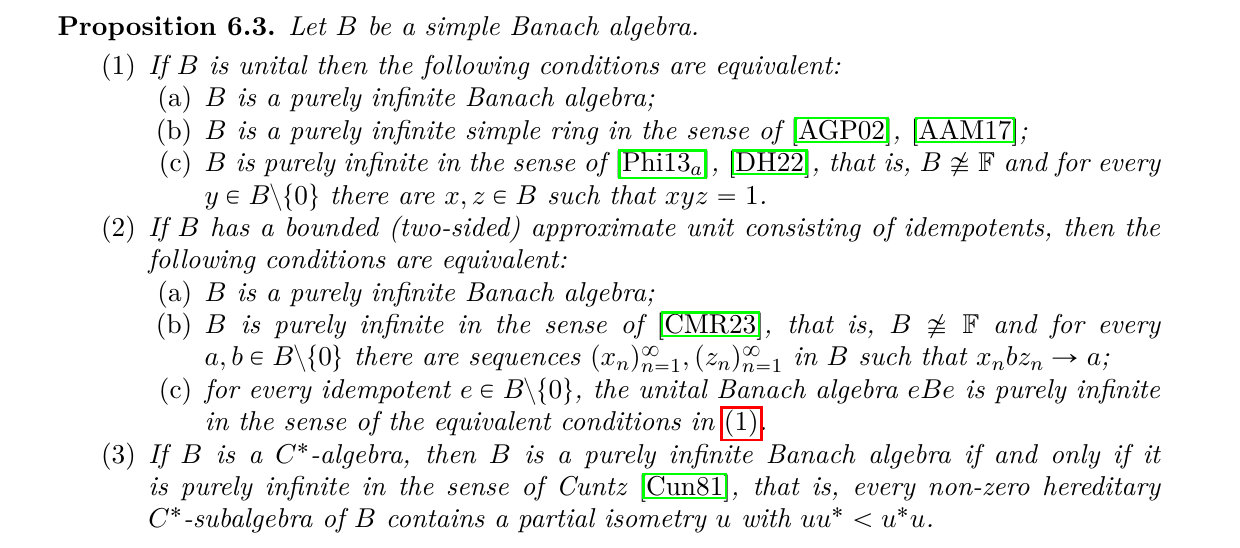
\includegraphics[width=0.96\textwidth]{figures/source_assumption_crop.png}
\caption{The standing approximate-unit hypothesis in source Proposition~6.3,
PDF page 27.}
\end{figure}

\begin{figure}[H]
\centering

\includegraphics[width=0.96\textwidth]{figures/open_problem_crop.png}
\caption{The open comparison in source Remark~6.4, PDF page 28.}
\end{figure}

The question may be transcribed as follows:

\begin{quote}
Without the bounded two-sided approximate-unit-of-idempotents assumption,
what is the relationship between the algebraic infinite-idempotent notion of
pure infiniteness and the sequential sandwich-approximation notion of
Corti\~nas--Montero--Rodr\'iguez?
\end{quote}

\section{Definitions}

All Banach algebras below are complex.  A Banach algebra $B$ is
\emph{topologically simple} if its only closed two-sided ideals are $0$ and
$B$.  Idempotents $e,f\in B$ are equivalent, written $e\sim f$, if
$e=uv$ and $f=vu$ for some $u,v\in B$.  An idempotent $e$ is
\emph{infinite} if it is equivalent to a proper sub-idempotent of itself.

For a topologically simple Banach algebra $B$, consider:

\begin{description}
\item[(API)] For every $b\in B\setminus\{0\}$, there are $x,z\in B$ such
that $xbz$ is an infinite idempotent.

\item[(SPI)] $B\not\cong\C$, and for every $b\in B\setminus\{0\}$ and
$a\in B$ there are sequences $(x_n)$ and $(z_n)$ in $B$ such that
$x_nbz_n\to a$.
\end{description}

(API) is Definition~6.1 of the source.  (SPI) is the simple pure-infiniteness
condition of Corti\~nas--Montero--Rodr\'iguez \cite{CMR}; allowing $a=0$
does not change it.

\section{Proof intuition}

There are two complementary mechanisms.  Under (API), factor an infinite
idempotent $e$ through a chosen nonzero $b$.  The corner $eBe$ is unital
purely infinite and hence properly infinite.  Its Cuntz families turn every
finite sum $\sum c_i e d_i$ into a \emph{single} sandwich $Ced$.
Topological simplicity makes such finite sums dense, giving (SPI).

Conversely, suppose (SPI) and retain only one nonzero idempotent $p$.  The CMR
corner theorem makes $pBp$ unital purely infinite, so $p$ itself is infinite.
Sequentially factor any nonzero $b$ toward $p$, compress to $pBp$, and use
openness of its invertible group to correct one sufficiently good
approximation to an exact factorization of $p$ through $b$.

The theorem therefore isolates the full unresolved issue: whether an (SPI)
Banach algebra can be idempotent-free.

\section{Exact characterization}

\begin{theorem}[The idempotent gap]
\label{thm:main}
Let $B$ be a complex topologically simple Banach algebra.  Then the following
are equivalent:
\begin{enumerate}
\item $B$ satisfies \emph{(API)};
\item $B$ satisfies \emph{(SPI)} and contains a nonzero idempotent.
\end{enumerate}
In particular, \emph{(API)} always implies \emph{(SPI)}, without any
approximate-identity hypothesis.
\end{theorem}

We use two established corner facts.  First, the source's proof of
Proposition~6.3 shows without any approximate-unit hypothesis that if $B$
satisfies (API) and $0\ne e=e^2\in B$, then $eBe$ is a unital purely infinite
Banach algebra \cite[Proposition~6.3(2), implication (a)$\Rightarrow$(c)]{BKM}.
Second, if $B$ satisfies (SPI), then every nonzero idempotent corner $eBe$ is
sequentially purely infinite and is not a division algebra
\cite[Lemmas~3.1--3.2 and Corollary~3.3]{CMR}.  A unital purely infinite
complex Banach algebra is properly infinite
\cite[Lemma~1.2]{DH}.

\begin{proof}
Assume first that $B$ satisfies (API), and fix $b\ne0$.  Choose $r,s\in B$
such that
\[
e=rbs
\]
is an infinite idempotent.  By the first corner fact, $eBe$ is a unital
purely infinite Banach algebra with unit $e$, hence $e$ is properly infinite.
Consequently, for every $m\ge1$ there are pairwise orthogonal idempotents
$e_1,\ldots,e_m\le e$, all equivalent to $e$.  Choose $u_i,v_i\in eBe$ so
that
\[
u_i v_i=e,\qquad v_i u_i=e_i.
\]
Orthogonality gives
\[
u_i v_j=u_i e_i e_jv_j=0\quad(i\ne j),
\qquad u_i v_i=e.
\tag{1}
\]

The closure of the algebraic ideal $BeB$ is a nonzero closed two-sided ideal,
so topological simplicity gives
\[
\overline{BeB}=B.
\tag{2}
\]
Given $a\in B$, choose finite sums
\[
a_n=\sum_{i=1}^{m_n}c_{n,i}e d_{n,i}\longrightarrow a.
\]
For a family satisfying (1) with $m=m_n$, set
\[
C_n=\sum_{i=1}^{m_n}c_{n,i}u_i,
\qquad
D_n=\sum_{i=1}^{m_n}v_i d_{n,i}.
\]
Then (1) yields
\[
C_neD_n=\sum_{i,j}c_{n,i}u_i v_jd_{n,j}
=\sum_i c_{n,i}e d_{n,i}=a_n.
\]
Since $e=rbs$, we have
\[
(C_nr)b(sD_n)=a_n\longrightarrow a.
\]
Thus $B$ satisfies (SPI).  It also contains the nonzero idempotent $e$.

Conversely, assume (SPI) and let $0\ne p=p^2\in B$.  By the second corner
fact, $pBp$ is a unital purely infinite Banach algebra; in particular its unit
$p$ is an infinite idempotent.  Fix $b\ne0$.  By (SPI), choose $x_n,z_n\in B$
such that $x_nbz_n\to p$.  In the unital Banach algebra $pBp$,
\[
w_n:=px_nbz_np\longrightarrow p.
\]
For some $n$, $w=w_n$ is invertible in $pBp$.  Therefore
\[
\bigl(w^{-1}px_n\bigr)b(z_np)=p.
\]
The right-hand side is an infinite idempotent, proving (API).
\end{proof}

\begin{corollary}
The unrestricted equivalence of (API) and (SPI) holds if and only if every
(SPI) complex Banach algebra contains a nonzero idempotent.  Any counterexample
to the equivalence must be idempotent-free.
\end{corollary}

\begin{proof}
The forward assertion is immediate from Theorem~\ref{thm:main}.  Conversely,
(API) itself produces a nonzero infinite idempotent, so an idempotent-free
(SPI) algebra cannot satisfy (API).
\end{proof}

\section{Scope, verification, and novelty}

The result is an exact characterization, but it does not decide whether the
extra idempotent condition follows automatically from (SPI).  Attempts using
approximate generalized inverses, unitization and spectral calculus,
primitive/radical structure, matrix amplification, and projectionless
examples did not remove that last condition.  In particular, (SPI) provides
approximations $x_nbz_n\to b$, not the regularity relation $by_nb\to b$
needed for standard idempotent perturbation arguments.

\paragraph{Verification notes.}
There is no computational dependency.  Review should focus on three points:
(i) the source's corner implication (API)$\Rightarrow$ unital pure
infiniteness of $eBe$ uses no approximate unit; (ii) proper infiniteness gives
the relations (1) for every finite size; and (iii) the CMR corner results make
$pBp$ unital purely infinite under (SPI).  The remaining steps are finite-sum
algebra and the Neumann-series openness of the invertible group of $pBp$.

\paragraph{Novelty check.}
On 11 August 2026, the four run indexes were searched for arXiv:2406.05717 and
the terms ``pure infiniteness'', ``CMR'', and ``idempotent''.  Bounded
arXiv/web searches used the exact source phrase and combinations of ``simple
purely infinite Banach algebra'', ``nonzero idempotent'', and ``approximate
unit''.  The source, CMR arXiv:2307.05555, and Daws--Horv\'ath
arXiv:2104.14989 were checked directly.  They contain the component corner and
proper-infiniteness facts, but no statement of Theorem~\ref{thm:main} was
located.  Novelty confidence is moderate because the combination is short and
may be folklore.

\paragraph{Human-review recommendation.}
Review as a substantial partial result.  It removes essentially all of the
source's approximate-unit hypothesis and identifies the exact residual
obstruction, but should not be presented as proving that (API) and (SPI) are
unconditionally equivalent.

\begin{thebibliography}{9}

\bibitem{BKM}
K.~Bardadyn, B.~Kwa\'sniewski, and A.~McKee,
\emph{Banach algebras associated to twisted \'etale groupoids: simplicity and
pure infiniteness}, arXiv:2406.05717, Proposition~6.3 and Remark~6.4.

\bibitem{CMR}
G.~Corti\~nas, D.~Montero, and M.~E.~Rodr\'iguez,
\emph{Simplicity of $L^p$-graph algebras}, arXiv:2307.05555,
Section~3.

\bibitem{DH}
M.~Daws and B.~Horv\'ath,
\emph{A purely infinite Cuntz-like Banach $*$-algebra with no purely infinite
ultrapowers}, J. Math. Anal. Appl. 514 (2022), 126241;
arXiv:2104.14989.

\end{thebibliography}

\end{document}
